\documentclass[a4paper,11pt,dvipdfmx]{ujarticle}
% パッケージ
\usepackage{graphicx}
\usepackage{url}
% レイアウト指定を記述したファイルの読み込み
\input{layout}

% タイトルと氏名を変更せよ．
\title{日本におけるデジタル化の状況}
\author{G684442026 川合陽向}

\begin{document}

\maketitle %ここにタイトルが入る
\section{デジタル競争力ランキング}
国際経営開発研究所(IDM)の調査\cite{imd}によると、日本のデジタル競争力のランキングは図1に示すように、調査対象の64カ国中、総合で28位、技術分野で30位となっている。
\begin{figure}[htbp]
    \centering
    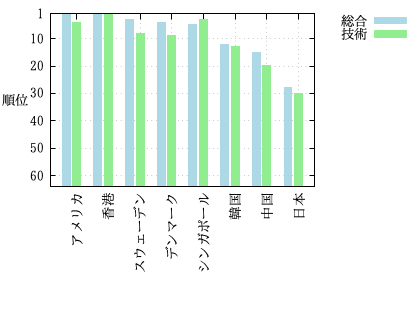
\includegraphics{fig41.png}
    \caption{図1：デジタル競争力ランキング(64カ国中)}
\end{figure}
\section{ブロードバンドの整備状況}
OECDによるブロードバンド回線の普及に関する調査\cite{oecd}によると、表1に示すように、日本における100人あたりの光ファイバー回線の加入者数は29.0で、韓国、スウェーデン、ノルウェーに続いて第4位になっている。
\begin{table}[htbp]
    \centering
    \caption{光ファイバー回線の加入者数(100人あたり)}
    \begin{tabular}{|c|c|c|}
        \hline
        順位　&国名&加入者数　\\
        \hline
        1位　&韓国&38.2 \\ 
        \hline
        2位　&スウェーデン&31.9 \\
        \hline
        3位　&ノルウェー&29.5 \\
        \hline
        4位　&日本&29.0 \\
        \hline
        5位　&アイスランド&28.8 \\
        \hline
        6位　&スペイン&27.3 \\
        \hline
        7位　&ポルトガル&25.1 \\
        \hline
        8位　&ニュージーランド&23.6 \\
        \hline
        9位　&リトアニア&22.3 \\
        \hline
        10位　&フランス&21.2 \\
        \hline
        
    \end{tabular}
\end{table}
\section{考察}
日本のブロードバンドの整備状況のランキングでは4位なのに、デジタル競争力ランキングでは28位と低いことから、整備されてはいるものの、設備を十分に生かしきれていないのではないか。


    % ここから本文
% 節見出し: \section{}
% を使う

% 本文(1)
%  参考文献の参照: \cite{}
%  図番号の参照： \ref{}
% を使う
% 文献データベースのキーワードは oecd と imd
% になっている．

% 図の挿入
% \includegraphics{}
% を
% \begin{figure}[htbp]
% \end{figure}
% で囲み
% \caption{}
% で図のタイトルを入れる．
% \label{}
% を使って図番号が参照できるようにする
% また，
% \centering
% で図が中央に来るようにする

% ーーー
% 節見出し(2)

% 本文(2)

% 表の挿入
% \begin{tabular}
% \end{tabular}    
% による表の記述を 
% \begin{table}[htbp]
% \end{table}
% で囲み
% \caption{}
% で表のタイトルを入れる．
% \label{}
% を使って表番号が参照できるようにする
% また，
% \centering
% で表が中央に来るようにする

% ーーー
% 見出し(3)
% 考察
%
% \begin{itemize}
% \end{itemize}
% を使って箇条書きで記述する

% ここに参考文献が入る

\bibliographystyle{junsrt}
\bibliography{exercise.bib}

\end{document}
